\subsection{DEM usado en pruebas preliminares}

\begin{figure}[H]
\centering
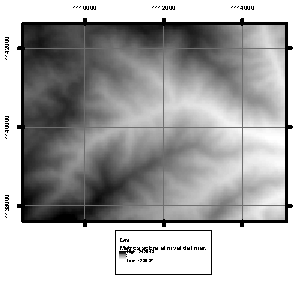
\includegraphics[scale=3]{dem.pdf}
\caption{Imagen monocrom\'atica del DEM trabajado desplegado en escala de grises. Altura m\'inima 1239 msnm, altura m\'axima 2425msnm. Elaboraci\'on propia.}
\label{fig:dem usado}
\end{figure}


Para las pruebas iniciales se us\'o el DEM mencionado en el numeral xxxxx de ASTER
GDEM V2 dada su f\'acil y r\'{a}pida adquisici\'on por medio del software Global Mapper
desarrollado por Blue Marvel.
El software Global Mapper tiene la capacidad de exportar el formato ESRI ASCII que utiliza
Scoops3D como insumo base, se recomienda exportar el DEM con la mayor resoluci\'{\o}n
posible, en caso de requerir agilizar el tiempo de procesamiento en Scoops3D, se
recomienda disminuir resoluci\'{\o}n espacial al DEM. Lo cual se puede lograr f\'{a}cilmente con la
herramienta Resample de ArcGIS en sus versiones 10 y superior (
Tool Geoprocessing
toolboxes $ (\setminus system toolboxes \setminus data management tools.tbx \setminus raster \setminus raster processing \setminus resample)$ y posteriormente la
herramienta \textbf{Raster to ASCII} $(toolboxes \setminus system toolboxes \setminus conversion tools.tbx \setminus from raster \setminus raster to ascii)$ en el software Qgis con la
herramienta Raster Calculator.\\
Debido a que Scoops3D no acepta sistemas de coordenadas geogr\'{a}ficas sino proyectadas,
se trabaj\'{\o} con el sistema de coordenadas MAGNA SIRGAS Colombia West zone. 
Se pudo comprobar que el idioma y la configuraci\'{\o}n regional puede causar que el archivo
DEM base pueda no ser compatible con Scoops3D debido al formato de separaci\'{\o}n de
decimales y unidades de miles. A continuaci\'{\o}n se muestra un archivo DEM incompatible y
uno compatible con Scoops 3D.

\begin{verbatim}
	   ncols 2
	   nrows 2
	   xllcorner 0
	   yllcorner 0
	   cellsize 1
	   NODATA_value -9999
	   0,5 1,5
	   2,5 -9999
\end{verbatim}

N\'{o}tese que la separaci\'{o}n de decimales se realiza con el car\'{a}cter coma (,). Esto como
resultado de la configuraci\'{o}n por defecto del sistema operativo Windows 10 en regiones
como am\'{e}rica latina y espa\~na.
Al introducir un archivo DEM con el formato anteriormente ejemplificado en Scoops3D, se
obtiene el siguiente error.


\newpage
\begin{verbatim}
	   ncols 2
	   nrows 2
	   xllcorner 0
	   yllcorner 0
	   cellsize 1
	   NODATA_value -9999
	   0.5 1.5
	   2.5 -9999
\end{verbatim}


El formato adecuado de DEM para usar con Scoops3D debe ser con separaci\'{o}n de
decimales con punto (.)
Finalmente se decidi\'{o} trabajar con un DEM de tama\~no de pixel 38m$\times$38m, esta es
resoluci\'{o}n obtenida de ASTER GDEM V2 sin modificaci\'on alguna para la zona de trabajo en el municipio de Ciudad Bol\'{i}var.
Este R\'aster se compone de 27.482 p\'ixeles, cubre en total \textbf{104.4 } hect\'areas,
comprende alturas entre los 1293 y los 2425 msnm.
En la zona de trabajo, con base en la informaci\'{o}n trabajada, se cuenta con laderas cuyas
pendientes alcanzan el 43 \%.

Dado que no se est\'a realizando el an\'alisis de una localidad especifica sino un \'area considerable, no se ha considerado necesario trabajar con cartograf\'ia de detalle. A manera de ensayo, se realiz\'o una corrida, con la misma extension del DEM mostrado en la figura \ref{fig:dem usado} y la misma configuraci\'on ilustrada en la figura \ref{fig:parameters}, empleando un DEM de tama\~no de pixel de 5x5 metros.
Bajo esta configuraci\'on la ejecuci\'on de Scoops3D se prolong\'o durante 30 horas sin obtener un resultado final.